The first round of testing was to ensure that the odometry was working properly; the first data set is the location dereived solely from odometry data.

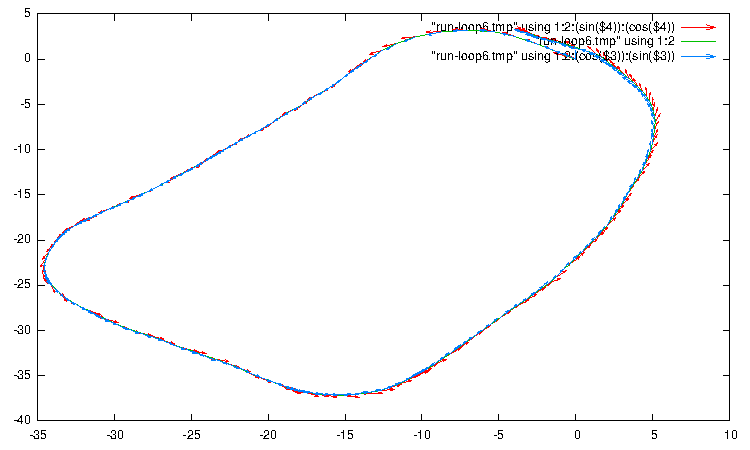
\includegraphics{run-loop6}

For the second round of testing, I wrote a program to give the robot four points in a square, so that it would drive in a roughly square-shaped pattern and return to its starting point. The data shows the robot's position estimate, including uncertainty, and the path plotted by raw odometry data.

TODO: gather actual path of robot and plot on graph.

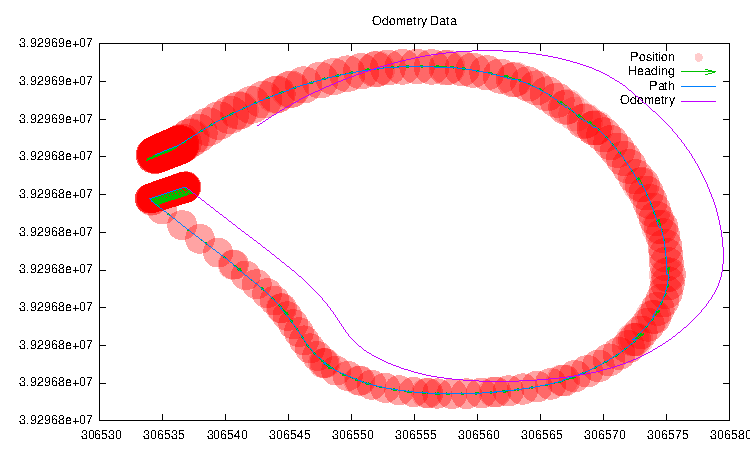
\includegraphics{run-2011-05-30-3}
